The total runtime of the algorithm on the image shown above for each number of processors:
\begin{figure}[H]
 \centering
 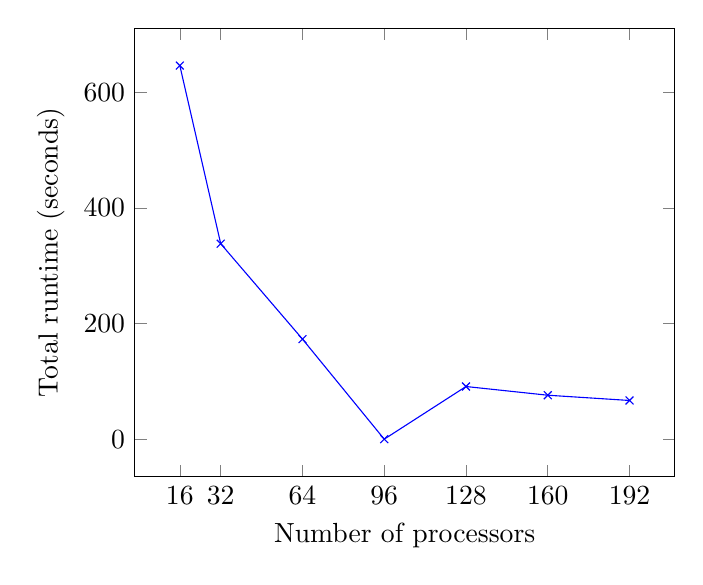
\begin{tikzpicture}
 \begin{axis}[
  xlabel=Number of processors,
  xtick={16, 32, 64, 96, 128, 160, 192},
  %xmode=log,
  %log ticks with fixed point,
  ylabel=Total runtime (seconds)]
   \addplot[color=blue, mark=x] coordinates {
    %(1, )
    %(2, )
    %(4, )
    %(8, )
    (16, 646.344379)
    (32, 338.1412974)
    (64, 173.1325498)
    (96, 0)
    (128, 91.1042946)
    (160, 76.0524958)
    (192, 66.9623342)
   };
 \end{axis}
\end{tikzpicture}

 \caption{Total runtime of the algorithm with entire matrix computation (log scale).}
 \label{fig:entire_runtime}
\end{figure}

We observe in figure \ref{fig:entire_runtime} that the runtime decreases significantly with respect to the number of processors.
We can also see that, by doubling the number of processors, we nearly accelerate the runtime by a factor 2.
It is an excellent result since we achieve strong scalability for the entire matrix computation case.
However, some overhead will always be present and the matrix-vector operations necessarily require communication, limiting scalability.
To deduce if some parts scale better than others, we compare the proportion of runtime spent in each part:
\begin{figure}[H]
 \centering
 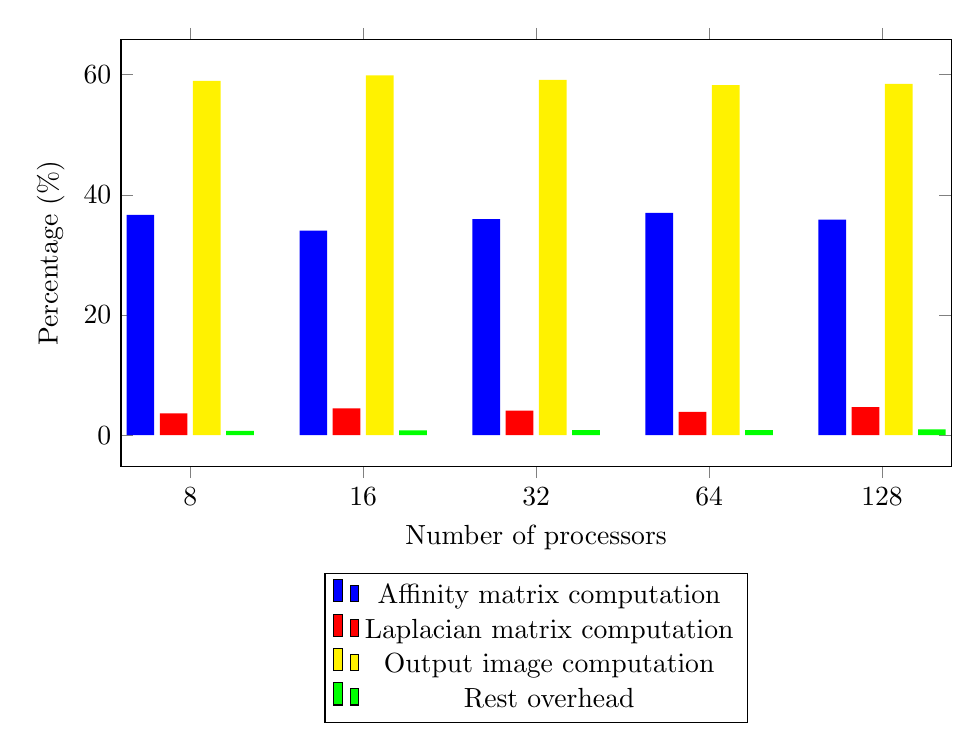
\begin{tikzpicture}
 \begin{axis}[
  ybar,
  height=7cm,
  width=\textwidth,
  xlabel=Number of processors,
  xtick={0, 1, 2, 3, 4},
  xticklabels={8, 16, 32, 64, 128},
  legend style={
   at={(0.5, -0.25)},
   anchor=north
  },
  ylabel={Percentage (\%)}]
  \addplot[draw=none, fill=blue] coordinates {
   (0, 36.67)
   (1, 34.04)
   (2, 35.96)
   (3, 37)
   (4, 35.88)};
  \addplot[draw=none, fill=red] coordinates {
   (0, 3.62)
   (1, 4.48)
   (2, 4.07)
   (3, 3.88)
   (4, 4.67)};
  \addplot[draw=none, fill=yellow] coordinates {
   (0, 58.99)
   (1, 59.9)
   (2, 59.15)
   (3, 58.26)
   (4, 58.48)};
  \addplot[draw=none, fill=green] coordinates {
   (0, 0.72)
   (1, 0.78)
   (2, 0.82)
   (3, 0.86)
   (4, 0.96)};
  \legend{
   Affinity matrix computation,
   Laplacian matrix computation,
   Output image computation,
   Rest overhead}
 \end{axis}
\end{tikzpicture}

 \caption{Proportion of runtime spent in each step in the total execution of the algorithm with entire matrix computation.}
 \label{fig:entire_proportion}
\end{figure}

We see in figure \ref{fig:entire_proportion} that the proportion of each part remains the same over the increase of processors, meaning that the three main parts scale equivalently.
However, when allocating an excessive amount of processors to this task compared to the input size, we may observe an increase of the runtime because we spend most time on communication overhead.

Overall, computing the entire matrices scales well because we only have matrix-matrix and matrix-vector products.
With an appropriate cluster, those scale nicely.
We now consider larger inputs, which require approximation and introduces linear algebra components which might slow down the algorithm.
